% usersguide.tex
%
%   make ug
%   evince userguide.pdf
%

\documentclass[10pt,a4paper]{article}

% same w/ Doxygen
%\documentclass[a4paper]{book}
\usepackage{a4wide}
\usepackage{makeidx}
\usepackage{fancyhdr}
%\usepackage{graphicx}
\usepackage{multicol}
\usepackage{float}
\usepackage{textcomp}
\usepackage{alltt}
\usepackage{times}
\usepackage[utf8]{inputenc}


% Listing for bash 
%   http://en.wikibooks.org/wiki/LaTeX/Packages/Listings
% Ubuntu texlive-latex-recommended package
%   /usr/share/texmf-texlive/tex/latex/listings
% Fedora texlive-texmf-latex-2007-34.fc12.noarch package
%   /usr/share/texmf/tex/latex/listings/
\usepackage{listings}

% Color?
%\usepackage{color}

%\makeindex
\setcounter{tocdepth}{3}
\renewcommand{\footrulewidth}{0.4pt}


\usepackage[dvipdfm]{graphicx, color}
%\usepackage{mediabb}

\usepackage{url}
% http://en.wikibooks.org/wiki/LaTeX/Hyperlinks
%\usepackage{hyperref}

% source code
% http://www.jorgemarsal.com/blog/2009/06/08/source-code-snippets-in-latex/
\usepackage{listings}
\definecolor{gray92}{gray}{.92}
\definecolor{gray88}{gray}{.88}
\definecolor{gray75}{gray}{.75}
\definecolor{gray45}{gray}{.45}
 
\lstdefinestyle{source_code}
{
numbers=none,
%stepnumber=5, 
%basicstyle=\normalsize, 
basicstyle=\footnotesize, 
captionpos = b, %bottom 
keywordstyle=\color[rgb]{0,0,1}, 
commentstyle=\color[rgb]{0.133,0.545,0.133}, 
stringstyle=\color[rgb]{0.627,0.126,0.941}, 
backgroundcolor=\color{gray92}, 
frame=lrtb, 
framerule=0.5pt, 
%linewidth = \textwidth 
linewidth = 170mm,
}

\lstdefinestyle{help_message}
{
numbers=none,
%stepnumber=5,
%basicstyle=\normalsize, 
basicstyle=\footnotesize, 
captionpos = b, %bottom 
keywordstyle=\color[rgb]{0,0,1},
commentstyle=\color[rgb]{0.133,0.545,0.133}, 
stringstyle=\color[rgb]{0.627,0.126,0.941}, 
backgroundcolor=\color{gray92}, 
frame=lrtb, 
framerule=0.5pt, 
%linewidth = \textwidth 
linewidth=170mm,
%framexleftmargin=-5mm
%framesep=10mm,
}


\lstdefinestyle{console} 
{ 
numbers=none,
%basicstyle=\bf\ttfamily,
basicstyle=\bf\footnotesize, 
backgroundcolor=\color{gray92},
%backgroundcolor=\color{gray88},
frame= lrtb, 
framerule=0.5pt, 
%linewidth=\textwidth, 
linewidth=170mm,
}


% size
\setlength{\textwidth}{170mm}
\setlength{\oddsidemargin}{-10mm}
\setlength{\evensidemargin}{-10mm}
\setlength{\topmargin}{-10mm}

\begin{document} 

\begin{titlepage}
\vspace*{7cm}
\begin{center}
{\Large Open Platform Trust Services (OpenPTS)\\User's Guide\\[1ex]\large Version 0.2.4}\\
\vspace*{1cm}
{\large Seiji Munetoh}\\
\vspace*{0.5cm}
{\small May 6, 2011}\\
%{\small \today}\\
\vspace*{2.0cm}
{\small Copyright @ 2011 IBM Corporation. All rights reserved}\\
{\small Mailing list for comments: openpts-users@lists.sourceforge.jp}\\
{\small Web access (preferred): http://sourceforge.jp/projects/openpts}\\
\end{center}
\end{titlepage}

%\clearemptydoublepage
\pagenumbering{roman}

\tableofcontents

\clearpage 
%\clearemptydoublepage
\pagenumbering{arabic}

%%%%%%%%%%%%%%%%%%%%%%%%%%%%%%%%%%%%%%%%%%%%%%%%%%%%%%%%%%%%%%%%%%%%%%%%%%%%%%
%%%%%%%%%%%%%%%%%%%%%%%%%%%%%%%%%%%%%%%%%%%%%%%%%%%%%%%%%%%%%%%%%%%%%%%%%%%%%%
\section{Introduction} 
%%%%%%%%%%%%%%%%%%%%%%%%%%%%%%%%%%%%%%%%%%%%%%%%%%%%%%%%%%%%%%%%%%%%%%%%%%%%%%
%%%%%%%%%%%%%%%%%%%%%%%%%%%%%%%%%%%%%%%%%%%%%%%%%%%%%%%%%%%%%%%%%%%%%%%%%%%%%%

\subsection{Purpose} 

The purpose of this User's Guide is to provide a description of
the usage of Open Platform Trust Services (OpenPTS).

\subsection{Scope} 

System administrator and developer of Trusted Platform.

\subsection{Architecture}

Figure \ref{fig:openpts-architecture} shows brief overview of OpenPTS architecture.
OpenPTS is used by both collector (target platform) and verifier sides.
Collector side, 'ptsc' command manages the integrity of target platform.
Verifier side, 'openpts' command is used to validate the target platform by remote attestation.
The protocol between ptsc and openpts is based on TCG IF-M protocol.
OpenPTS uses SSH between collector and verifier to secure the remote attestation.
This figure shows stand-alone operation mode.
OpenPTS supports IMC and IMV interfaces for TNC (Trusted Network Connect).

% pdftops -eps OpenPTS-fig-architecture.pdf
\begin{figure}[hb!p]
  \begin{center}
    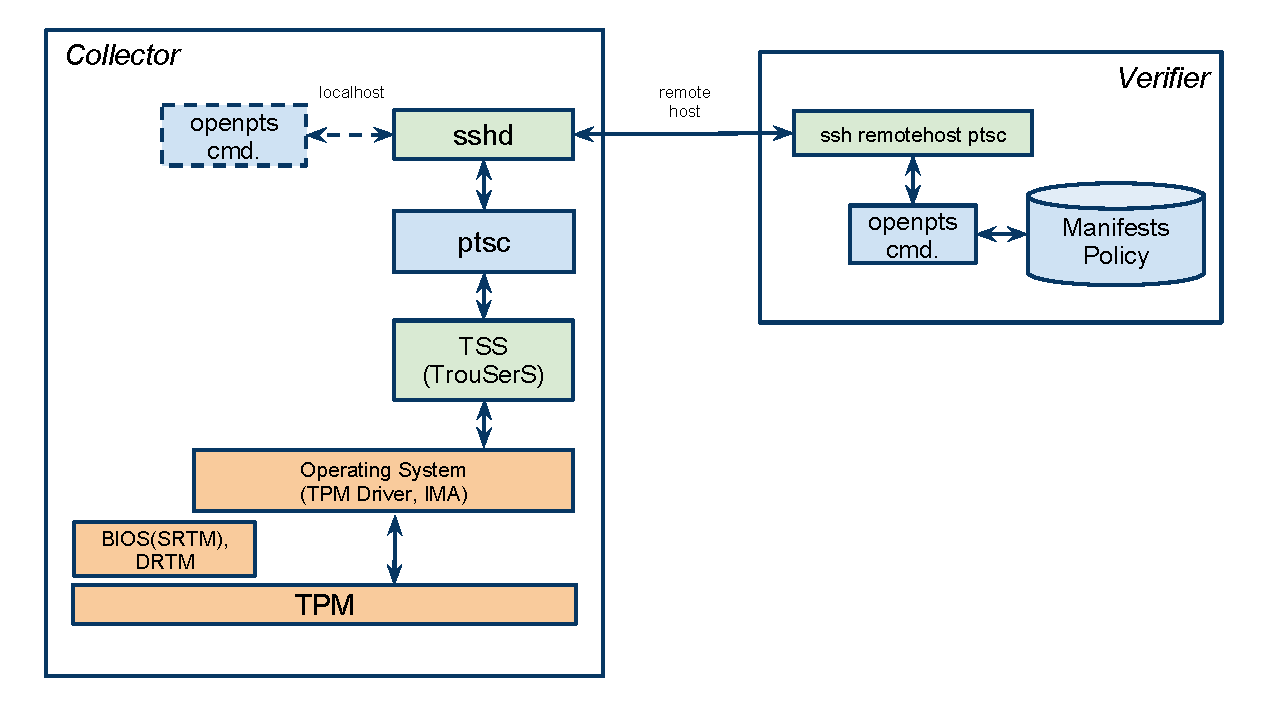
\includegraphics[width=15cm]{OpenPTS-fig-architecture.eps}
  \end{center}
  \caption{OpenPTS - Architecture (Standalone Mode)}
  \label{fig:openpts-architecture}
\end{figure}



\clearpage
\subsection{Operations}

Figure \ref{fig:openpts-dataflow} shows how OpenPTS manage the integrity.
OpenPTS uses a model which describe the behavior of transitive trust chain of target platform.
The model is Finite State Machine (FSM) written by UML state diagram.
OpenPTS uses this model to parse the integrity measurement log (IML)
and generate the reference manifest (RM).

The behavior model just describe the general behavior of transitive trust chain and is used to generate RM and integrity report (IR).
OpenPTS supports generic model of x86(PC) platform.
The binary model contains actual digest value of target and used to validate the IML.

By using the model, we can translate the binary measurement (hash value) into security properties.
%hen, translated properties are validated by given policies to get the final result,
%VALID/INVALID/UNKNOWN.
Therefore we can use a policy to validate the property.
This provides a flexible management of target platform.
Finally, we get the validation result, VALID/INVALID/UNKNOWN.


% pdftops -eps OpenPTS-fig-dataflow.pdf
\begin{figure}[hb!p]
  \begin{center}
    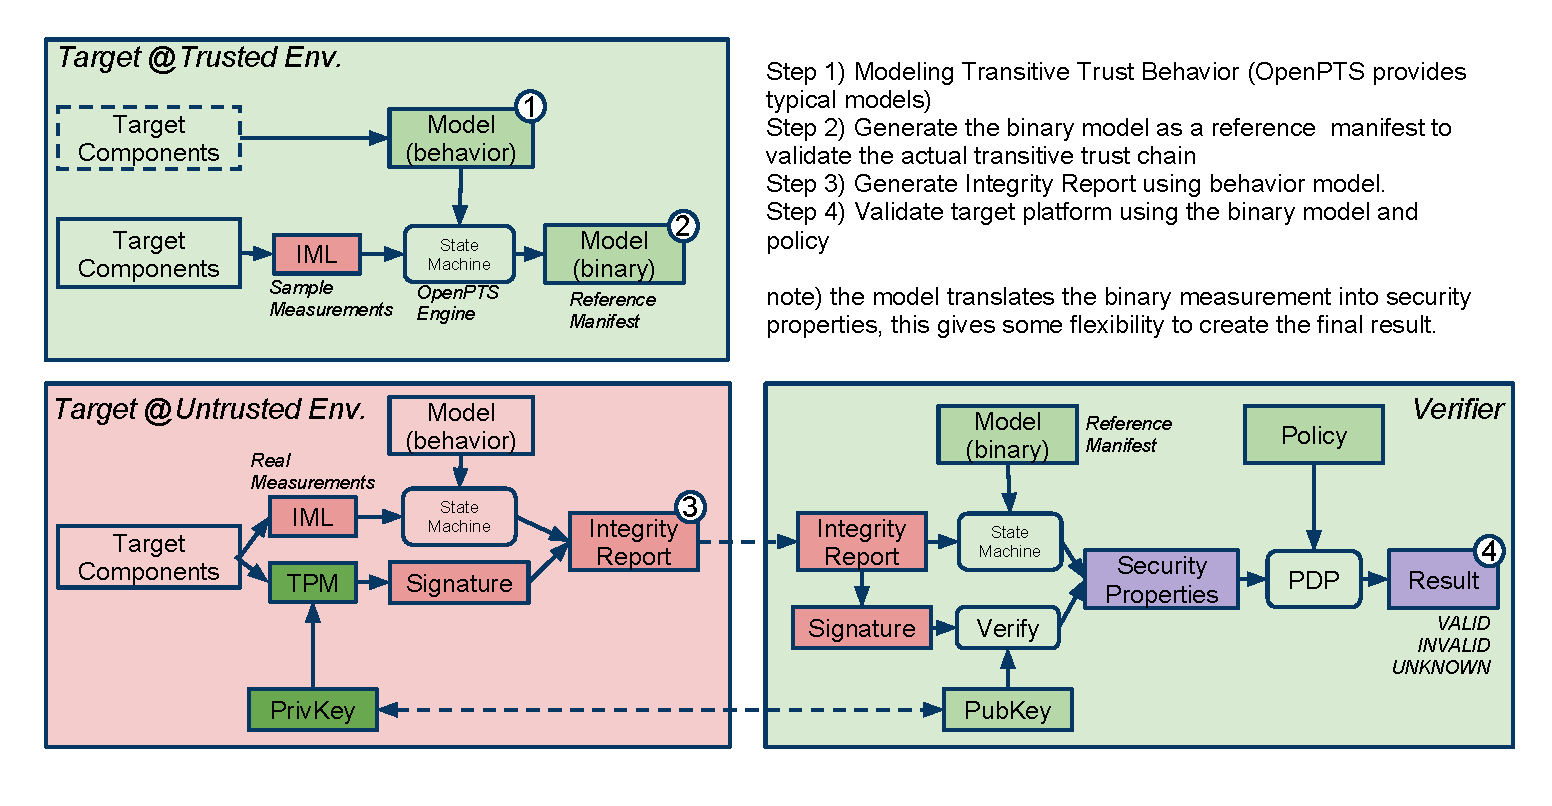
\includegraphics[width=15cm]{OpenPTS-fig-dataflow.eps}
  \end{center}
  \caption{OpenPTS - Integrity Management Flow}
  \label{fig:openpts-dataflow}
\end{figure}

\subsection{Limitation}

\begin{itemize}
\item AIDE and TNC integration is still under development.
\item Need to apply the patch to TrouSerS (TSS) to handle eventlog properly.
\item 
There is no interoperability of standalone IF-M mode between version 0.2.3 and 0.2.4
since we had changed this operation from version 0.2.4.
Version 0.2.3 used ptscd daemon and SSH tunnel.
This was deprecated since the management of SSH tunnel did not scale.
Now we use simple SSH remote command execution.
The IF-M go through the pipe between collector(ptsc command) and verifier(openpts command) protected by SSH.
\end{itemize} 



%%%%%%%%%%%%%%%%%%%%%%%%%%%%%%%%%%%%%%%%%%%%%%%%%%%%%%%%%%%%%%%%%%%%%%%%%%%%%%
%%%%%%%%%%%%%%%%%%%%%%%%%%%%%%%%%%%%%%%%%%%%%%%%%%%%%%%%%%%%%%%%%%%%%%%%%%%%%%
\clearpage
\section{Use case 1. Standalone Remote Attestation}



In this use case,
We use individual reference manifest and integrity database for each target platform.
Thus, the reference manifest and integrity database are created by collector running at the target platform.
Fig \ref{fig:openpts-selfupdate} shows the operation flow of OpenPTS.


%\begin{figure}[b!p]
%  \begin{center}
%    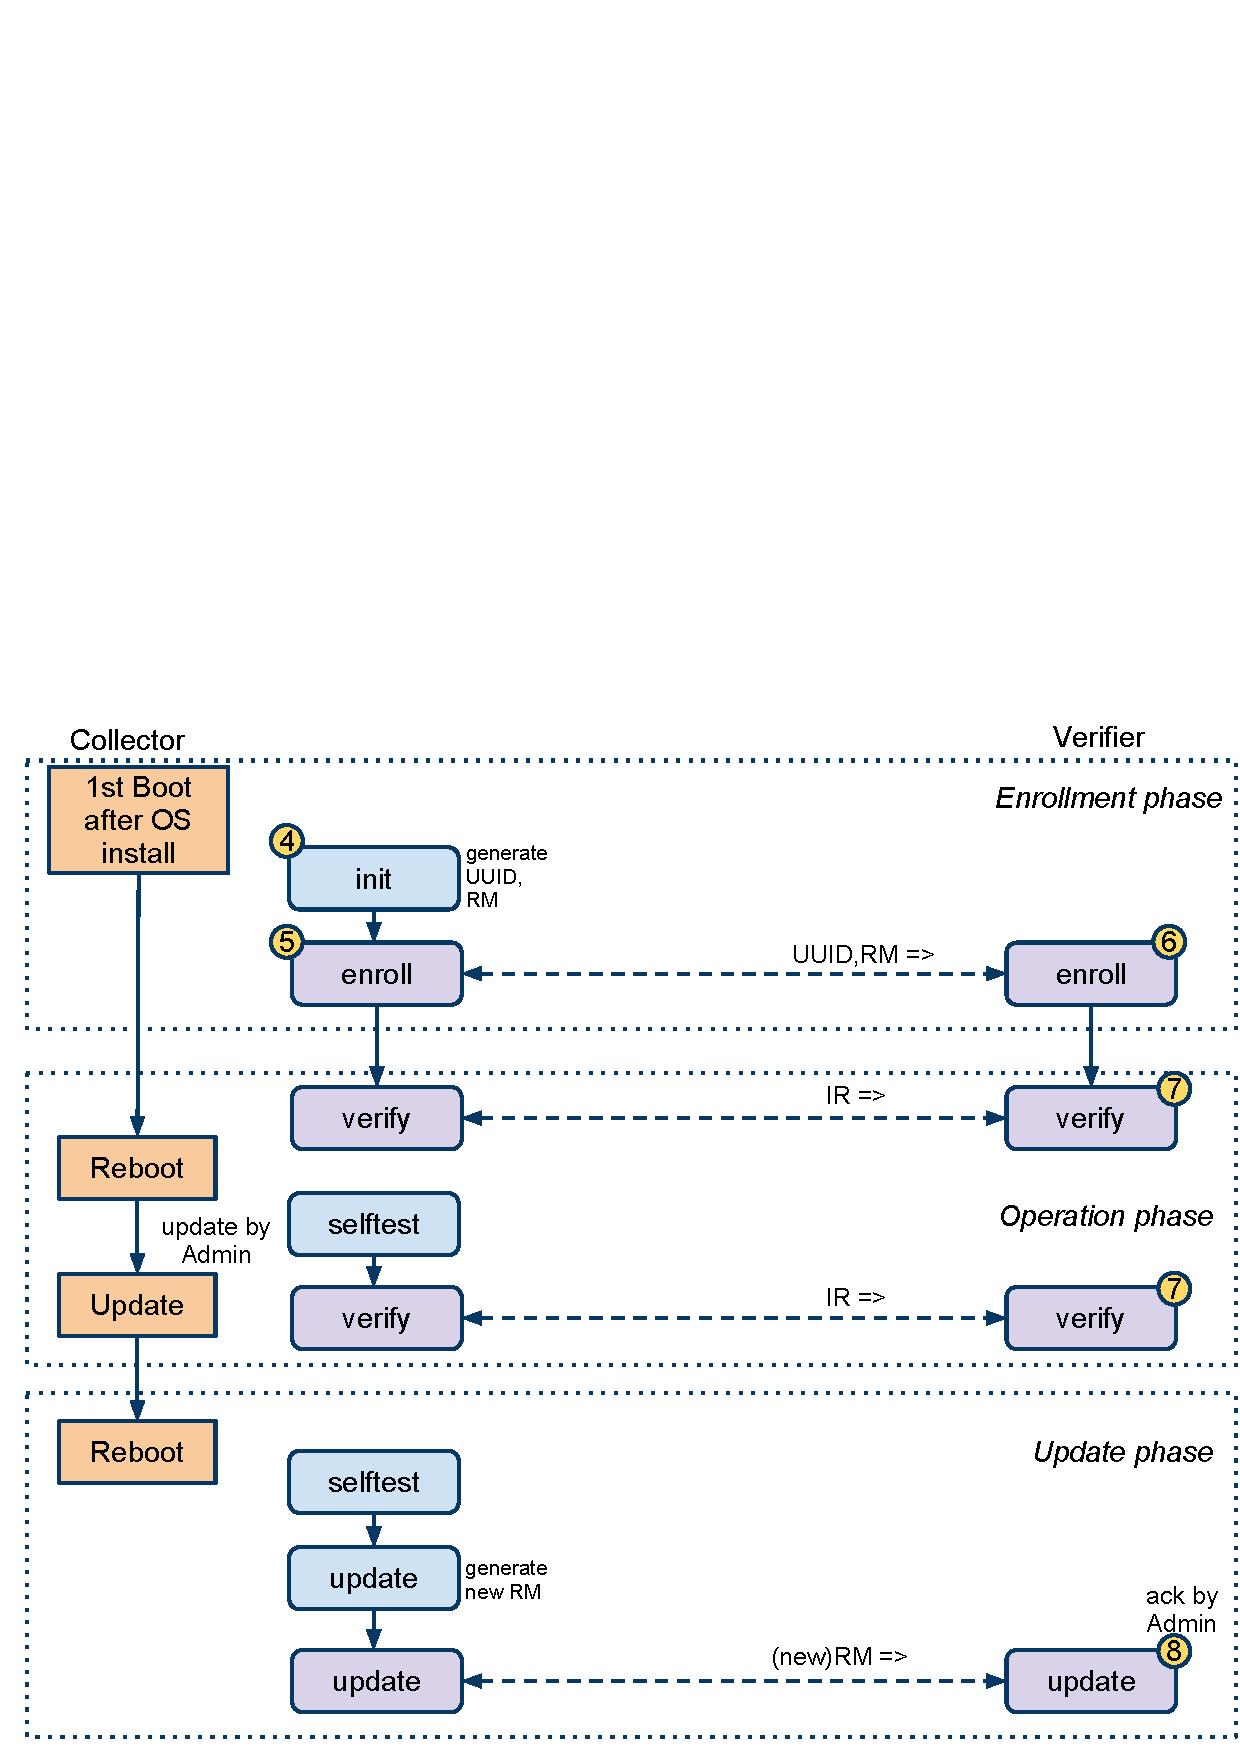
\includegraphics[width=15cm]{OpenPTS-fig-selfupdate.png}
%  \end{center}
%  \caption{TNC mode}
%  \label{fig:openptstnc}
%\end{figure}

% png - NG on Fedora 12
% pdf to eps
% yum install xpdf  - NG :-(
% pdftoeps -eps OpenPTS-fig-selfupdate.pdf -NG :-(
% yum install poppler-utils
% pdftops -eps OpenPTS-fig-selfupdate.pdf

\begin{figure}[hb!p]
  \begin{center}
    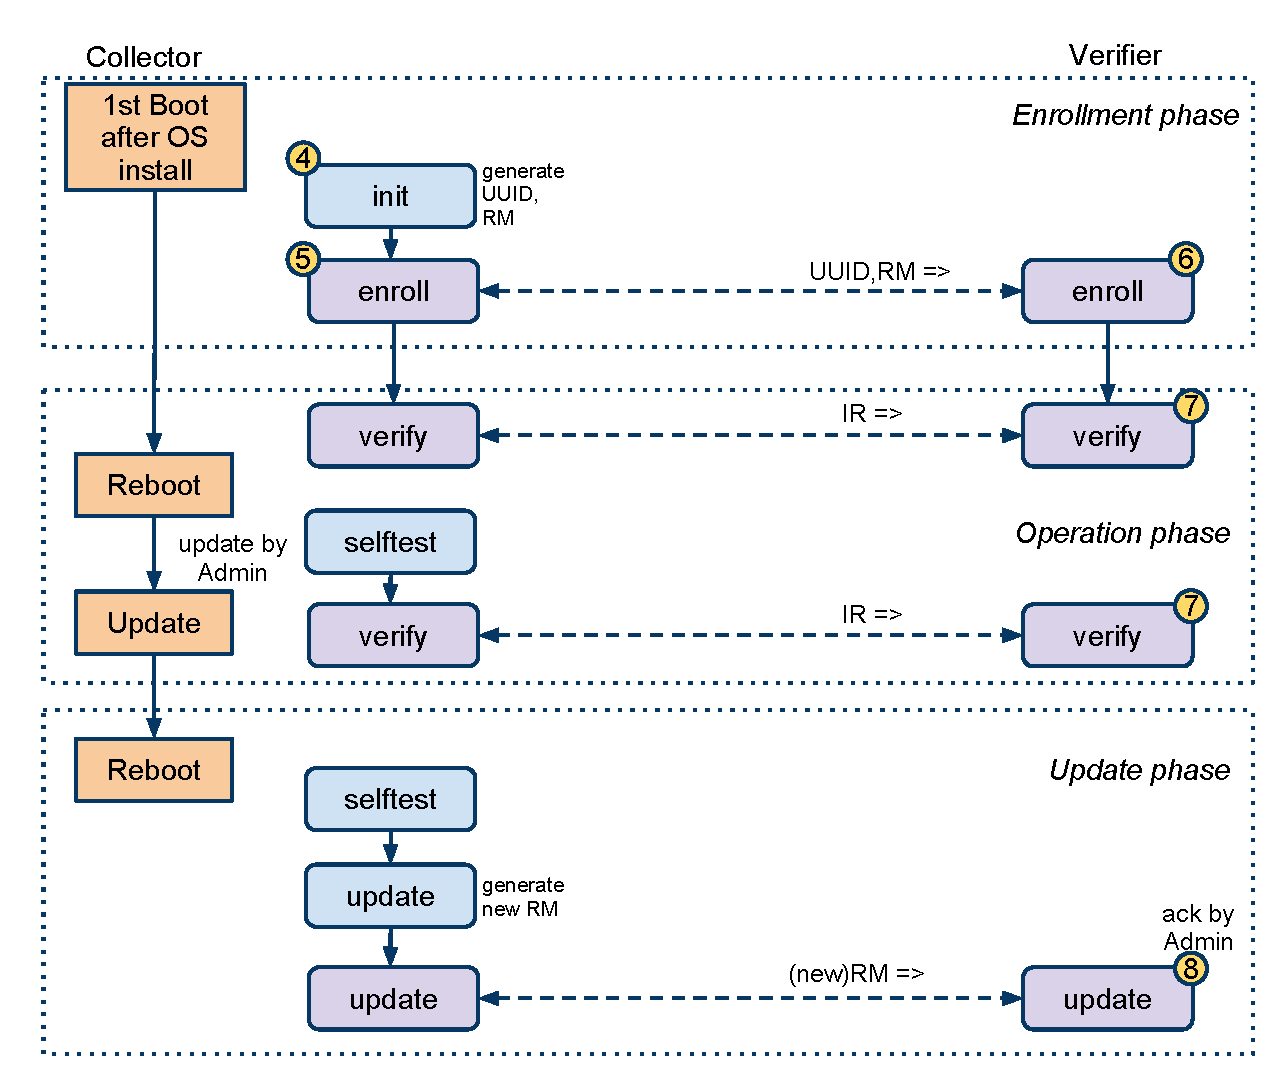
\includegraphics[width=15cm]{OpenPTS-fig-selfupdate.eps}
  \end{center}
  \caption{OpenPTS - Operation Flow}
  \label{fig:openpts-selfupdate}
\end{figure}


This use case have three operation phases as follows.

\begin{description}
\item[Enrollment phase]
We trust an installation process\footnote{If we have the EK credential of TPM, we can trust the remote platform}.
The collector generate the new UUID to identify the target and reference manifest based on the measurement of initial boot.
Thus, the reference manifests are based on actual BIOS
\footnote{OpenPTS generate manifest of actual measurement since there are no PC and BIOS vendors which disclose integrity information.}
and Operating System measurement at this phase. Verifier get the UUID and manifests from the Collector and securely stored them.

\item[Operation phase]
Verifier validate the target (remote attestation).

\item[Update phase]
After the BIOS or OS update, manifest must be updated.
The OpenPTS collector do selftest at the startup run (ptsc -s).
If validation was failed due to the change, it generates the new manifest.

If the update was expected, Verifier update the manifest too.

\end{description}

\begin{description}
 \item[Enrollment]  Initial setup (Trusted environment)
 \item[Operation]   Status check by Remote Attestation (Untrusted environment)
 \item[Update]      Update the SW status (Trusted environment)
\end{description}

\subsection{Setup the Collector (target platform)}

\subsubsection{Take the TPM ownerdhip}

Take ownership of your TPM with well known secret.

\begin{lstlisting}[style=console] 
# tpm_takeownership -y -z
\end{lstlisting}

\subsubsection{Install openpts}

(see the section 7, how to build) \\
\begin{lstlisting}[style=console]
# rpm -ivh openpts-0.2.4-1.x86_64.rpm
\end{lstlisting}

\subsubsection{Configure ptsc}

After the installation, adjust the configuration file '/etc/ptsc.conf'
If you are using GRUB-IMA, assign the validation models to PCR[4,5,8].
\begin{lstlisting}[style=source_code]
rm.num=2
rm.model.1.pcr.4=grub_pcr4hdd.uml
rm.model.1.pcr.5=grub_pcr5.uml
rm.model.1.pcr.8=grub_pcr8.uml
\end{lstlisting}
If you enabled Linux-IMA, assign the validation model of IMA to PCR[10].
\begin{lstlisting}[style=source_code]
rm.model.1.pcr.10=f12_ima_pcr10.uml
\end{lstlisting}
Set the platform infomation. e.g.
\begin{lstlisting}[style=source_code]
platform.system.manufacturer=LENOVO
platform.system.productname=745749J
platform.system.version=ThinkPad X200
platform.bios.version=6DET58WW
\end{lstlisting}
The platform infomation stored in SMBIOS can be checked by 'dmidecode' command.

\subsubsection{Setup the AIDE database (OPTIONAL)}
Create the sample AIDE DB from current IML.
(It takes long time).
\begin{lstlisting}[style=console] 
# iml2aide -c /etc/ptsc.conf -o /var/lib/aide/aide.db.gz
\end{lstlisting}
Or create the AIDE DB.
(It takes long time too).
\begin{lstlisting}[style=console]
# cp /usr/share/openpts/aide.conf  /etc/aide.conf
# aide -i
\end{lstlisting}

\subsubsection{Initialize Collector ptsc}

e.g.
\begin{lstlisting}[style=console]
 # /usr/sbin/ptsc -i
 Generate uuid               : 186bebba-2781-11e0-bcdb-001f160c9c28 
 Sign key  location          : SYSTEM
 Generate UUID (for RM)      : 19566e16-2780-11e0-bf2e-001f160c9c28 
 level 0 Reference Manifest  : /var/lib/openpts//19566e16-...9c28/rm0.xml
 level 1 Reference Manifest  : /var/lib/openpts//19566e16-...9c28/rm1.xml
\end{lstlisting}

Selftest the target platform.
\begin{lstlisting}[style=console]
 # /usr/sbin/ptsc -t
 selftest - OK
\end{lstlisting}

\subsubsection{Startup ptsc}
\begin{lstlisting}[style=console]
 # service ptsc start
 Starting ptsc:                                            [  OK  ]
\end{lstlisting}

Also, set whether ptsc should run on startup.

\begin{lstlisting}[style=console]
 # chkconfig --add ptsc
\end{lstlisting}

%\end{description}


Setup of the PTS collector is done.


\subsection{Setup the Verifier} 

Install openpts to the localhost (or any remote verifier box).

\subsubsection{Install openpts}

Use the same package, it contains both collector and verifier.

\begin{lstlisting}[style=console]
 # rpm -ivh openpts-0.2.4-1.x86_64.rpm
\end{lstlisting}


\subsubsection{Setup SSH pub-key authentication}

You have to setup SSH public key authentication between collector and verifier.
The following example uses foo@localhost as the target (collector).
e.g.
\begin{lstlisting}[style=console]
 $ ssh-keygen -t rsa
 $ ssh-copy-id foo@localhost
\end{lstlisting}


\subsubsection{Enrollment with Collector}

First, you enroll the collector.
e.g.
\begin{lstlisting}[style=console]
 $ openpts -i localhost
 /usr/bin/openpts -i -l foo localhost
 /home/foo/.openpts is missing. create [Y/n]:Y
 Target            : localhost
 Collector UUID    : 186bebba-2781-11e0-bcdb-001f160c9c28
 Manifest UUID     : 19566e16-2780-11e0-bf2e-001f160c9c28
 manifest[0]       : /home/foo/.openpts/186bebba-...9c28//19566e16-...9c28/rm0.xml
 manifest[1]       : /home/foo/.openpts/186bebba-...c9c28//19566e16-...c9c28/rm1.xml
 configuration     : /home/foo/.openpts/186bebba-...9c28/target.conf
 validation policy : /home/foo/.openpts/186bebba-...9c28/policy.conf
\end{lstlisting}
target.conf, policy.conf (and aide.ignore) are automaticaly generated.
rm0.xml, rm1.xml and aide.db.gz are received from collector.
To override existing setting, use "-f" option.
\begin{lstlisting}[style=console]
 $ openpts -i -f localhost
\end{lstlisting}
See the Table \ref{table:openpts:file} about the file used by openpts command.

%\end{description}
%
%\subsection{Remote Attatation (localhost)} 
%\begin{description}
\subsubsection{Remote Attestation}

\begin{lstlisting}[style=console]
 $ openpts -v localhost
 Target         : localhost
 Collector UUID : 186bebba-2781-11e0-bcdb-001f160c9c28
 Manifest UUID  : 19566e16-2780-11e0-bf2e-001f160c9c28
 username(ssh)  : default
 port(ssh)      : default
 policy file    : /home/foo/.openpts/186bebba-...9c28/policy.conf
 property file  : /home/foo/.openpts/186bebba-...9c28/vr.properties
 integrity      : valid
\end{lstlisting}

%\end{description}


\subsection{Collector update the manifests} 


At the startup, the collector selftest the platform.
If the seftest was faild, the collector generate the new manifest against current measurements.
This happen if you update any relevent components, such as the BIOS or OS image.

\subsection{Verifier update the manifests} 

\subsubsection{Accept the change happen on the collector}

When the collector update the manifest, 
verification of the target was fail since there are mismatch between the collector and the verifier.
\begin{lstlisting}[style=console]
 $ openpts -v localhost
 Target         : localhost
 Collector UUID : 1dbac28e-2787-11e0-b84a-001f160c9c28
 Manifest UUID  : 1df210fe-2787-11e0-b84a-001f160c9c28
 port           : 6678 (localhost)
 policy file    : /home/foo/.openpts/1dbac28e-2787-11e0-b84a-001f160c9c28/policy.conf
 property file  : /home/foo/.openpts/1dbac28e-2787-11e0-b84a-001f160c9c28/vr.properties
 integrity      : unknown (INTERNAL ERROR) rc=35
 Reasons
     0 Missing Reference Manifest(RM)
     1 Collector hostname = localhost
     2 Collector UUID = 1dbac28e-2787-11e0-b84a-001f160c9c28
     3 Collector RM UUID = 33b88c38-2787-11e0-adc0-001f160c9c28
 New reference manifest exist. if this is expected change, update the manifest by openpts -i -f 
\end{lstlisting}
If this is predicted or legitimate change. Update the target information.
\begin{lstlisting}[style=console]
 $ openpts -i -f  localhost
 Target            : localhost
 Collector UUID    : 1dbac28e-2787-11e0-b84a-001f160c9c28
 Manifest UUID     : 33b88c38-2787-11e0-adc0-001f160c9c28
 manifest[0]       : /home/foo/.openpts/1dbac28e-...c9c28//33b88c38-...9c28/rm0.xml
 manifest[1]       : /home/foo/.openpts/1dbac28e-...9c28//33b88c38-...9c28/rm1.xml
 configuration     : /home/foo/.openpts/1dbac28e-...9c28/target.conf
 validation policy : /home/foo/.openpts/1dbac28e-...9c28/policy.conf
\end{lstlisting}
Then verify again.
\begin{lstlisting}[style=console]
 $ openpts -v localhost
 Target         : localhost
 Collector UUID : 1dbac28e-2787-11e0-b84a-001f160c9c28
 Manifest UUID  : 33b88c38-2787-11e0-adc0-001f160c9c28
 username(ssh)  : default
 port(ssh)      : default
 policy file    : /home/foo/.openpts/1dbac28e-...9c28/policy.conf
 property file  : /home/foo/.openpts/1dbac28e-...9c28/vr.properties
 integrity      : valid
\end{lstlisting}


\subsection{Check the status}

\subsubsection{Status of the collector}

\begin{lstlisting}[style=console]
# /usr/sbin/ptsc -D
openpts version 0.2.2.svn

config file                 : /etc/ptsc.conf
UUID                        : 186bebba-...c9c28 (/var/lib/openpts/uuid)
IML access mode             : TSS
  Runtime IML type          : IMA (kernel 2.6.32)
RM UUID (current)           : 19566e16-2780-11e0-bf2e-001f160c9c28
RM UUID (for next boot)     : (null)
List of RM set              : 1 RM set in config dir
                               ID  UUID                 date(UTC)         status
                              -------------------------------------------------------
                                0 d5086d88-...c9c28 2011-01-24-05:50:21 state=UNKNOWN
                              -------------------------------------------------------
Integrity Report            : /var/lib/openpts/ir.xml
Model dir                   : /usr/share/openpts/models
                              Behavior Models
                              PCR lv  FSM files
                              -----------------------------------------------------
                               0  0  /usr/share/openpts/models/bios_pcr0.uml
                               1  0  /usr/share/openpts/models/bios_pcr1.uml
                               2  0  /usr/share/openpts/models/bios_pcr2.uml
                               3  0  /usr/share/openpts/models/bios_pcr3.uml
                               4  0  /usr/share/openpts/models/bios_pcr4.uml
                               4  1  /usr/share/openpts/models/grub_pcr4hdd.uml
                               5  0  /usr/share/openpts/models/bios_pcr5.uml
                               5  1  /usr/share/openpts/models/grub_pcr5.uml
                               6  0  /usr/share/openpts/models/bios_pcr6.uml
                               7  0  /usr/share/openpts/models/bios_pcr7.uml
                               8  1  /usr/share/openpts/models/grub_pcr8.uml
                              10  1  /usr/share/openpts/models/f12_ima_pcr10.uml
                              -----------------------------------------------------
\end{lstlisting}

\subsubsection{Status of the verifier}
\begin{lstlisting}[style=console]
$ openpts -D
Show openpts config
--------------------------------------------------------------------
config file               : /home/foo/.openpts/openpts.conf
uuid                      : 240fbb66-6fdb-11e0-a735-001f160c9c28
--------------------------------------------------------------------
target[0] uuid            : cf9cfa32-6fba-11e0-84de-001f160c9c28
target[0] config          : /home/foo/.openpts/cf9cfa32-6fba-11e0-84de-001f160c9c28/target.conf
target[0] hostname        : localhost
--------------------------------------------------------------------
target[1] uuid            : 0445a354-6fdb-11e0-aa91-001f160c9c28
target[1] config          : /home/foo/.openpts/0445a354-6fdb-11e0-aa91-001f160c9c28/target.conf
target[1] hostname        : host023
--------------------------------------------------------------------
\end{lstlisting}
%\end{description}


%%%%%%%%%%%%%%%%%%%%%%%%%%%%%%%%%%%%%%%%%%%%%%%%%%%%%%%%%%%%%%%%%%%%%%%%%%%%%%
%%%%%%%%%%%%%%%%%%%%%%%%%%%%%%%%%%%%%%%%%%%%%%%%%%%%%%%%%%%%%%%%%%%%%%%%%%%%%%

%%%%%%%%%%%%%%%%%%%%%%%%%%%%%%%%%%%%%%%%%%%%%%%%%%%%%%%%%%%%%%%%%%%%%%%%%%%%%%
%%%%%%%%%%%%%%%%%%%%%%%%%%%%%%%%%%%%%%%%%%%%%%%%%%%%%%%%%%%%%%%%%%%%%%%%%%%%%%
%\clearpage
%\section{Usecase 2. Common Remote Attestation - TBD}
%In this usecase we use common Integrity Database to validate the IMA measurment.
Version 0.2.1 did not support this usecase. It will be supported in later version.

\subsection{Setup IIDB} 

\subsection{Setup the target (collector) platform} 

\subsection{Setup the verifier} 

\subsection{Remote Attestation} 

\subsection{Update IIDB} 


%%%%%%%%%%%%%%%%%%%%%%%%%%%%%%%%%%%%%%%%%%%%%%%%%%%%%%%%%%%%%%%%%%%%%%%%%%%%%%
%%%%%%%%%%%%%%%%%%%%%%%%%%%%%%%%%%%%%%%%%%%%%%%%%%%%%%%%%%%%%%%%%%%%%%%%%%%%%%
%In this use case we use common Integrity Database to validate the IMA measurment.
%Version 0.2.2 did not support this usecase. It will be supported in the later version.




%%%%%%%%%%%%%%%%%%%%%%%%%%%%%%%%%%%%%%%%%%%%%%%%%%%%%%%%%%%%%%%%%%%%%%%%%%%%%%
%%%%%%%%%%%%%%%%%%%%%%%%%%%%%%%%%%%%%%%%%%%%%%%%%%%%%%%%%%%%%%%%%%%%%%%%%%%%%%
\clearpage
\section{OpenPTS Commands Usage} 
\lstset{frame=trbl}
\lstset{language=}
\lstset{commentstyle=\textit}
\lstset{basicstyle=\small}

\subsection{ptsc} 

PTS collector.

\begin{lstlisting}[style=help_message]
Usage: ptsc [options] [command]

Commands: (forgrand)
  -i                    Initialize PTS collector
  -t                    Self test (attestation)
  -s                    Startup (selftest + timestamp)
  -u                    Update the RM
  -U                    Update the RM (auto)
  -D                    Display the configuration
  -m                    IF-M mode

Miscellaneous:
  -h                    Show this help message
  -v                    Verbose mode. Multiple -v options increase the verbosity.

Options:
  -c configfile         Set configuration file. defalt is /etc/ptsc.conf
  -P name=value         Set properties.
  -R                    Remove RMs
  -z                    Use the SRK secret to all zeros (20 bytes of zeros)
\end{lstlisting}


\subsection{openpts} 

PTS verifier.

\begin{lstlisting}[style=help_message]
Usage: openpts [options] {-i [-f]|[-v]|-D} <target>
       openpts -D

Commands:
  -i [-f]               Initialize [forcibly] the PTS verifier with the target(collector).
  [-v]                  Verify target(collector) integrity against know measure.
  -D                    Display the configuration (target/ALL)

Miscellaneous:
  -h                    Show this help message
  -V                    Verbose mode. Multiple -V options increase the verbosity.

Options:
  -u                    Selects 'yes' as the the default answer when an update is available [no]
  -l username           ssh username [ssh default]
  -p port               ssh port number [ssh default]
  -c configfile         Set configuration file [~/.openpts/openpts.conf]
\end{lstlisting}

\subsection{uml2dot} 

Generate dot file from the UML State Diagram model.

\begin{lstlisting}[style=help_message]
Usage: uml2dot [options] umlfile

Options
   -o output	        Set output file (default is stdout)

Example:
$ uml2dot -o pcr0.dot pcr0.uml
$ dot -Tpng pcr0.dot -o pcr0.png
$ eog pcr0.png
\end{lstlisting}

\subsection{rm2dot} 

Generate dot file from Reference Manifest (RM).
Select pcr index since the RM may contains multiple FSMs for each PCRs. 

\begin{lstlisting}[style=help_message]
Usage: rm2dot [options] rmfile

Options
	-o output	set output file (default is stdout)
	-p pcrindex	set PCR index
	-l level	set snapshot level (0 or 1)

Example:
$ rm2dot -p 0 -o pcr0.dot rm.uml
$ dot -Tpng pcr0.dot -o pcr0.png
$ eog pcr0.png
\end{lstlisting}

\subsection{iml2text} 

Dump the eventlog in text.
It take out the eventlog from TSS or securityfs file directly.

\begin{lstlisting}[style=help_message]
Usage: iml2text [options]

Options:
  -i filename           Set binary eventlog file (at securityfs)
  -p pcr_index          Select pcr (TSS)
  -I mode               Select IMA's log format (Kernel 2.6.32:32)
  -V                    Verify
  -D                    DRTM
  -E                    Enable endian conversion (BE->LE or LE->BE)
  -h                    Show this help message


Example:
$ iml2text
 Idx PCR       Type    Digest                                EventData
-----------------------------------------------------------------------
   0   0 0x00000008 1dfce7dde0cf13cfff102b1eb01875f752d5090c [BIOS:EV...
   1   0 0x00000001 1c41801dd329198e50a3d98040230095693e49b3 [BIOS:EV...
   2   0 0x00000001 16fb111792cb98a3de12f3abd0406fc04c7e5fca [BIOS:EV...
   3   0 0x00000001 dd261ca7511a7daf9e16cb572318e8e5fbd22963 [BIOS:EV...
<snip>
\end{lstlisting}

\subsection{iml2aide} 

Convert IML to AIDE database.

\begin{lstlisting}[style=help_message]
Usage: iml2aide [option]

Options:
  -c filename           Set config file
  -i filename           Set IMA IML file. default, get IML via TSS
  -r filename           Set AIDE DB file as reference of fullpathname
  -o filename           Set output file (AIDE DB format, gziped)
  -w filename           Set output file (Ignore name list, plain text format)
  -h                    Show this help message

Example:
$ src/iml2aide -c /etc/ptsc.conf -r /var/lib/aide/aide.db.new.gz \
  -o /tmp/aide.db.gz
  AIDE DB(ref) : 241826 entries (/var/lib/aide/aide.db.new.gz)
  IML          : 5681 events (TSS)
  AIDE DB      : 3986 entries (tests/data/Fedora12/aide.db.gz) 
\end{lstlisting}


\subsection{ir2text}

Convert Integrity Report (IR) to text format or binary format (=IML).

\begin{lstlisting}[style=help_message]
Usage: ir2text [options]

Options:
  -i filename           Set IR file
  -o filename           Set output file, else stdout
  -P filename           Set PCR output file (option)
  -b                    Binary, (Convert IR to IML)
  -E                    Enable endian conversion (BE->LE or LE->BE)
  -h                    Show this help message
\end{lstlisting}

\subsection{tboot2iml}

Convert the tboot messages to IML.

\begin{lstlisting}[style=help_message]
Usage: tboot2iml [options]

Options:
  -i filename           txt-stat file to read (default is STDIN)
  -g filename           grub.conf file to read (OPTION)
  -p path               grub path (OPTION)
  -o filename           Output to file (default is STDOUT)
  -v                    Verbose message
  -h                    Help

Example:
  # txt-stat >  txt-stat
  # tboot2iml -i txt-stat >> binary_rtm_measurments

\end{lstlisting}




%%%%%%%%%%%%%%%%%%%%%%%%%%%%%%%%%%%%%%%%%%%%%%%%%%%%%%%%%%%%%%%%%%%%%%%%%%%%%%
%%%%%%%%%%%%%%%%%%%%%%%%%%%%%%%%%%%%%%%%%%%%%%%%%%%%%%%%%%%%%%%%%%%%%%%%%%%%%%
\clearpage
\section{OpenPTS Configuration Files} 


\subsection{Files}

OpenPTS generates and uses many files as described below.
Table \ref{table:ptsc:file} lists the files used by collector (ptsc command).
Table \ref{table:openpts:file} lists the files used by verifier (openpts command).
The verifier store the target infomation at the user's home directory.

\begin{table}[h]
\caption{Files - collector side, (ptsc command)}
\label{table:ptsc:file}
\begin{center}
%\begin{tabular}{|l|l|}
\begin{tabular}{ll}
        \hline
        File & Description  \\
        \hline  \hline
        /etc/ptsc.conf  &  configuration file of collector \\
        \hline
        /var/lib/openpts/uuid     &   uuid of this platform \\
        \hline
        /var/lib/openpts/rm\_uuid &   uuid of current manifest (=RM\_UUID)\\
        \hline
        /var/lib/openpts/newrm\_uuid &   uuid of next boot-cycle manifest (=NEWRM\_UUID) TBD\\
        \hline
        /var/lib/openpts/\{RM\_UUID\}/rm0.xml &  Reference Manifest (BIOS) \\
        \hline
        /var/lib/openpts/\{RM\_UUID\}/rm1.xml &  Reference Manifest (IPL and OS) \\
        \hline
        /var/lib/aide/aide.db.gz    &  AIDE database file \\
        \hline
        /tmp/.ptsc/openpts/\{VERIFIER\_UUID\}\_\{IR\_UUID\}.xml &  Integrity Reports of each attestation\\
        \hline
\end{tabular}
\end{center}
\end{table}

\begin{table}[h]
\caption{Files - verifier side (openpts command)}
\label{table:openpts:file}
\begin{center}
%\begin{tabular}{|l|l|}
\begin{tabular}{ll}
        \hline
        File & Description  \\
        \hline  \hline
        HOME/.openpts/openpts.conf &  configuration file of verifier\\
        \hline
        HOME/.openpts/\{COLLECTOR\_UUID\}/target.conf &  configuration file of each target \\
        \hline
        HOME/.openpts/\{COLLECTOR\_UUID\}/policy.conf &  validation policy \\
        \hline
        HOME/.openpts/\{COLLECTOR\_UUID\}/ir.xml &  Integrity Report (XML) \\
        \hline
        HOME/.openpts/\{COLLECTOR\_UUID\}/vr.properties &  target properties \\
        \hline
        HOME/.openpts/\{COLLECTOR\_UUID\}/\{RM\_UUID\}/rm0.xml &  Reference Manifest (BIOS)  (XML)\\
        \hline
        HOME/.openpts/\{COLLECTOR\_UUID\}/\{RM\_UUID\}/rm1.xml &  Reference Manifest (IPL and OS)  (XML)\\
        \hline
        HOME/.openpts/\{COLLECTOR\_UUID\}/aide.db.gz &  AIDE database as Integrity Database \\
        \hline
        HOME/.openpts/\{COLLECTOR\_UUID\}/aide.ignore &  list of valid components not listed on AIDE database \\
        \hline
\end{tabular}
\end{center}
\end{table}


\clearpage
\subsection{/etc/ptsc.conf} 

\begin{table}[h]
\caption{/etc/ptsc.conf}
\label{table:ptsc:conf}
\begin{center}
\begin{tabular}{lll}
    \hline
    Name & Value & Description  \\
    \hline  \hline
    config.dir & /var/lib/openpts & Set location of ptsc data \\
    \hline
    srk.password.mode & known & SRK password is well known secret (20 bytes of zeros)\\
                      & null  & SRK password is null,  SHA1("")\\
    \hline
    iml.mode & tss        & Get IML via TSS \\
             & securityfs & Get IML from securityfs filesystem \\
    \hline
    runtime.iml.type & IMA32 &  kernel 2.6.32 \\
    \hline
    rm.num & 1 & Number of manifest.\\
    & & 1: Platform only\\
    & & 2: Platform and Runtime\\
    \hline
    rm.basedir & /var/lib/openpts/ & Dir for Manifests\\
    ir.dir & /tmp/.ptsc & Dir for Integrity Reports\\
    %ir.file & /var/lib/openpts/ir.xml & \\
    uuid.file & /var/lib/openpts/uuid & UUID of Collector\\
    rm.uuid.file & /var/lib/openpts/rm\_uuid & UUID of Manifest\\
    newrm.uuid.file & /var/lib/openpts/newrm\_uuid & UUID of new Manifest\\
    model.dir & /usr/share/openpts/models & Dir of validation models\\
    \hline
    rm.model.0.pcr.0 & bios\_pcr0.uml & validation model of BIOS PCR[0], CRTM\\
    rm.model.0.pcr.1 & bios\_pcr1.uml & validation model of BIOS PCR[1]\\
    rm.model.0.pcr.2 & bios\_pcr2.uml & validation model of BIOS PCR[2], OPTION ROM\\
    rm.model.0.pcr.3 & bios\_pcr3.uml & validation model of BIOS PCR[3]\\
    rm.model.0.pcr.4 & bios\_pcr4.uml & validation model of BIOS PCR[4], IPL\\
    rm.model.0.pcr.5 & bios\_pcr5.uml & validation model of BIOS PCR[5]\\
    rm.model.0.pcr.6 & bios\_pcr6.uml & validation model of BIOS PCR[6]\\
    rm.model.0.pcr.7 & bios\_pcr7.uml & validation model of BIOS PCR[7]\\
    \hline
    rm.model.1.pcr.4 & grub\_pcr4hdd.uml & validation model of GRUB PCR[4], IPL\\
    rm.model.1.pcr.5 & grub\_pcr5.uml & validation model of GRUB PCR[5], IPL data\\
    rm.model.1.pcr.8 & grub\_pcr8.uml & validation model of GRUB PCR[8], OS images\\
    \hline
    rm.model.1.pcr.10 & ima\_pcr10.uml & validation model of Linux-IMA\\
    \hline
    rm.model.1.pcr.11 & openpts.uml & validation model of OpenPTS\\
    \hline
    platform.system.manufacturer & & \\
    platform.system.productname & & \\
    platform.system.version & & \\
    platform.bios.version & & \\
    \hline
    runtime.vendor.name & redhat & \\
    runtime.distro.name & rhel & \\
    runtime.distro.version & 6 & \\
    \hline
\end{tabular}
\end{center}
\end{table}

\clearpage
\subsection{~/.openpts/openpts.conf} 

\begin{table}[h]
\caption{~/.openpts/openpts.conf}
\label{table:openpts:conf}
\begin{center}
\begin{tabular}{lll}
    \hline
    Name & Value & Description  \\
    \hline  \hline
uuid.file & ./uuid & \\
verifier.logging.dir & ./ & \\
    \hline
\end{tabular}
\end{center}
\end{table}

\subsection{~/.openpts/UUID/target.conf} 

\begin{table}[h]
\caption{~/.openpts/UUID/target.conf}
\label{table:target:conf}
\begin{center}
\begin{tabular}{lll}
    \hline
    Name & Value & Description  \\
    \hline  \hline
hostname & (hostname) & Target hostname\\
port & 6678 & Target port\\
\hline
ssh.mode & on & Use SSH tunnel\\
         & off & direct access (localhost)\\
\hline
ssh.username & (foo) & SSH account name\\
ssh.port & (6680) & SSH tunneling port\\
\hline
target.uuid & & UUID string \\
target.pubkey & (base64) & Publik Key \\
\hline
ima.validation.mode & none & \\
\hline
rm.num & 1 or 2 & Number of Manifest\\
rm.basedir & ./ & \\
rm.uuid.file & ./rm\_uuid & \\
newrm.uuid.file & ./newrm\_uuid & \\
oldrm.uuid.file & ./oldrm\_uuid & \\
ir.file & ./ir.xml & \\
prop.file & ./vr.properties & \\
policy.file & ./policy.conf & \\
verifier.logging.dir & ./ & \\
\hline

    \hline
\end{tabular}
\end{center}
\end{table}



%%%%%%%%%%%%%%%%%%%%%%%%%%%%%%%%%%%%%%%%%%%%%%%%%%%%%%%%%%%%%%%%%%%%%%%%%%%%%%
%%%%%%%%%%%%%%%%%%%%%%%%%%%%%%%%%%%%%%%%%%%%%%%%%%%%%%%%%%%%%%%%%%%%%%%%%%%%%%
\clearpage
\section{Configulation of Trusted Platform}
Unfortunately, There is no Linux distribution which configure the Trusted Platform well.


\begin{table}[h]
\caption{Linux distribution and TC support}
\label{table:ptsc:file}
\begin{center}
%\begin{tabular}{|l|l|l|l|l|l|}
\begin{tabular}{llllll}
        \hline
        OS        & Kernel & CONFIG\_IMA & IPL & SRTM & DRTM \\
        \hline  \hline
        Fedora 12        & 2.6.32 & Yes & Grub-0.97 & patch & NA \\
        \hline
        Fedora 13        & 2.6.34 & Yes & Grub-0.97 & patch & NA \\
        \hline
        Fedora 14        & 2.6.35 & Yes &      &       & tboot \\
        \hline
        Fedora 15        & 2.6.38 & Yes &      &       & tboot \\
        \hline
        RHEL 6.0         & 2.6.32 & Yes & Grub-0.97 &  & NA \\
        \hline
        Ubuntu 10.04 LTS & 2.6.32 & No  & Grub2 & NA & NA \\
        \hline
        Ubuntu 10.10     & 2.6.35 & No  & Grub2 & NA & OK \\
        \hline
\end{tabular}
\end{center}
\end{table}

\subsection{RHEL 6.0 - SRTM}

SRTM based Trusted Boot (BIOS, no UEFI) and IMA could be enabled.

\subsubsection{GRUB-IMA} 

Download source code "grub-0.97-68.el6.src.rpm" and patch.

\begin{lstlisting}[style=console, linewidth = 170mm]
$ su -c 'yum install ncurses-devel ncurses-static gnu-efi glibc-static \
  glibc-devel-2.12-1.7.el6_0.3.i686 glibc-static-2.12-1.7.el6_0.3.i686'
$ rpm -Uvh grub-0.97-68.el6.src.rpm
$ cd ~/rpmbuild/SOURCES
$ wget http://osdn.dl.sourceforge.jp/openpts/40294/grub-0.97-68.el6.ima-1.1.0.0.patch
$ cd ~/rpmbuild/SPECS
\end{lstlisting}

Modify grub.spec file as follows.

\begin{lstlisting}[style=source_code]
Release: 68%{?dist}.ima
<snip>
Patch32: grub-0.97-68.el6.ima-1.1.0.0.patch
<snip>
%patch32 -p1
<snip>
%configure --sbindir=/sbin --disable-auto-linux-mem-opt \
--enable-ima --datarootdir=%{_datadir}
\end{lstlisting}

Build the RPM and intall.

\begin{lstlisting}[style=console, linewidth = 170mm]
$ rpmbuild -ba grub.spec
$ su -c 'rpm -ivh ../RPMS/x86_64/grub-0.97-68.el6.ima.x86_64.rpm'
$ su -c 'grub-install /dev/sda'
$ grep TCG /boot/grub/*
Binary file /boot/grub/stage1 matches
Binary file /boot/grub/stage2 matches
\end{lstlisting}

\subsubsection{Linux IMA} 

Add option "ima=on" at the kernel line in /boot/grub/grub.conf file.
If you have Intel TPM (Thinkpad X200, T400 etc), you also need additional options.
Add tpm\_tis.itpm=1 tpm\_tis.force=1 tpm\_tis.interrupts=0 ima=on at the kernel line
Set SELinux to permissive mode. System->Admin->SELinux management
if you don't have /sys/kernel/security/ direcroty, please add following line to /etc/fstab

\begin{lstlisting}[style=source_code]
    * securityfs /sys/kernel/security securityfs rw 0 0 
\end{lstlisting}

\subsubsection{TrouSetS(TSS)}

TrouSerS is provided by RedHat.
However, you have to use the latest TrouSerS
since trousers-0.3.4-4.el6.x86\_64 do not support the eventlog created by Linux-IMA.

\begin{lstlisting}[style=source_code]
$ git clone git://trousers.git.sourceforge.net/gitroot/trousers/trousers trousers-git
$ cd trousers-git
$ sh bootstrap.sh
$ ./configure
$ cd ..
$ ln -s trousers-git trousers-0.3.6git
$ tar zcvf ~/rpmbuild/SOURCES/trousers-0.3.6git.tar.gz ./trousers-0.3.6git/*
$ rpmbuild -bb trousers-0.3.6git/dist/trousers.spec

# rpm -ivh --force trousers-0.3.6git-1.x86_64.rpm
\end{lstlisting}

notes) You may need to fix the package dependancies in trousers.spec


Modify /etc/tcsd.conf file as follows

\begin{lstlisting}[style=source_code]
firmware_log_file = /sys/kernel/security/tpm0/binary_bios_measurements
kernel_log_file = /sys/kernel/security/ima/binary_runtime_measurements
firmware_pcrs = 0,1,2,3,4,5,6,7,8
kernel_pcrs = 10
\end{lstlisting}

notes) if you already taken the ownership and the system.data is missing. please copy the dummy system.data.

\begin{lstlisting}[style=source_code]
cp ./dist/dummy\_tss\_system.data /var/lib/tpm/system.data
\end{lstlisting}

Ok, enable tcsd daemon.

\begin{lstlisting}[style=source_code]
chkconfig tcsd on
service tcsd start
\end{lstlisting}


\subsection{Fedora 12 - SRTM} 

SRTM based Trusted Boot and IMA could be enabled.

\subsubsection{GRUB-IMA} 

Download source code and patch.

\begin{lstlisting}[style=console, linewidth = 170mm]
$ su -c 'yumdownloader --source grub'
$ su -c 'yum-builddep grub-0.97-62.fc12.src.rpm'
$ rpm -Uvh grub-0.97-62.fc12.src.rpm
$ cd ~/rpmbuild/SOURCES
$ wget http://osdn.dl.sourceforge.jp/openpts/40294/grub-0.97-62.fc12.ima-1.1.0.0.patch
$ cd ~/rpmbuild/SPECS
\end{lstlisting}

Modify grub.spec file as follows.

\begin{lstlisting}[style=source_code]
+Release: 62%{?dist}.ima
+Patch2: grub-0.97-62.fc12.ima-1.1.0.0.patch
+%patch2 -p1
+%configure --sbindir=/sbin --disable-auto-linux-mem-opt \
--enable-ima --datarootdir=%{_datadir}
\end{lstlisting}

Build the RPM and intall.

\begin{lstlisting}[style=console, linewidth = 170mm]
$ rpmbuild -ba grub.spec
$ su -c 'rpm -ivh ../RPMS/x86_64/grub-0.97-62.fc12.ima.x86_64.rpm'
$ su -c 'grub-install /dev/sda'
\end{lstlisting}

\subsubsection{Linux IMA} 

Add option "ima\_tcb=1" at the kernel line in /boot/grub/grub.conf file.

If you have Intel TPM (Thinkpad X200, T400 etc), you also need additional options.

Add tpm\_tis.itpm=1 tpm\_tis.force=1 tpm\_tis.interrupts=0 ima\_tcb=1 at the kernel line

Set SELinux to permissive mode. System->Admin->SELinux management

if you don't have /sys/kernel/security/ direcroty, please add following line to /etc/fstab

\begin{lstlisting}[style=source_code]
    * securityfs /sys/kernel/security securityfs rw 0 0 
\end{lstlisting}

\subsubsection{TrouSetS(TSS)}

Modify /etc/tcsd.conf file as follows

\begin{lstlisting}[style=source_code]
firmware_log_file = /sys/kernel/security/tpm0/binary_bios_measurements
kernel_log_file = /sys/kernel/security/ima/binary_runtime_measurements
firmware_pcrs = 0,1,2,3,4,5,6,7,8
kernel_pcrs = 10
\end{lstlisting}

\subsection{Fedora 15 - SRTM and DRTM} 

The target platform must support Intel TXT.
This example uses Lenovo Thinkpad X200.
Note that this is experimental support 
and configulation of the tboot may differ according to the hardware.

\subsubsection{Configure tboot}

tboot did not support well known secret against the ownership.
\begin{lstlisting}[style=source_code]
tpm_takeownership -z
\end{lstlisting}

\begin{lstlisting}[style=source_code]
# yum install tboot
\end{lstlisting}
Change /boot/grub/grub.conf
\begin{lstlisting}[style=source_code]
title Fedora (2.6.38.1-6.fc15.x86_64) tboot
        root (hd0,0)
        kernel /tboot.gz logging=serial,vga,memory vga_delay=5
        module /vmlinuz-2.6.38.1-6.fc15.x86_64 ro root=/dev/mapper/vg_munetohx200f15-lv_root \
        rd_LVM_LV=vg_munetohx200f15/lv_root rd_LVM_LV=vg_munetohx200f15/lv_swap rd_NO_LUKS \
        rd_NO_MD rd_NO_DM LANG=en_US.UTF-8 SYSFONT=latarcyrheb-sun16 KEYTABLE=us selinux=0 \
        rhgb quiet xdriver=vesa nomodeset 1
        module /initramfs-2.6.38.1-6.fc15.x86_64.img
        module /GM45_GS45_PM45_SINIT_21.BIN
\end{lstlisting}
Create LCP policy
\begin{lstlisting}[style=source_code]
# cd /root
# lcp_mlehash -c "logging=serial,vga,memory vga_delay=5" /boot/tboot.gz > mle_hash
# lcp_crtpol -t hashonly -m mle_hash -o lcp.pol
\end{lstlisting}

\begin{lstlisting}[style=source_code]
$ tb_polgen --create --type nonfatal vl.pol
\end{lstlisting}

\begin{lstlisting}[style=source_code]
$ tb_polgen --add --num 0 --pcr none --hash image --cmdline "ro \
  root=/dev/mapper/vg_munetohx200f15-lv_root rd_LVM_LV=vg_munetohx200f15/lv_root \
  rd_LVM_LV=vg_munetohx200f15/lv_swap rd_NO_LUKS rd_NO_MD rd_NO_DM \
  LANG=en_US.UTF-8 SYSFONT=latarcyrheb-sun16 KEYTABLE=us selinux=0 rhgb quiet \
  xdriver=vesa nomodeset 1" --image /boot/vmlinuz-2.6.38.1-6.fc15.x86_64 vl.pol
\end{lstlisting}

\begin{lstlisting}[style=source_code]
$ tb_polgen --add --num 1 --pcr 19 --hash image --cmdline "" --image \
  /boot/initramfs-2.6.38.1-6.fc15.x86_64.img vl.pol
\end{lstlisting}

\begin{lstlisting}[style=source_code]
$ tpmnv_defindex -i 0x20000002 -s 8 -pv 0 -rl 0x07 -wl 0x07 -p TPM-password
$ tpmnv_defindex -i owner -p TPM-password
$ tpmnv_defindex -i owner -s 34 -pv 0x02 -p TPM-password
$ tpmnv_defindex -i 0x20000001 -s 256 -pv 0x02 -p TPM-password
\end{lstlisting}

\begin{lstlisting}[style=source_code]
$ tpmnv_getcap
  The response data is:
  20 00 00 02 20 00 00 01 40 00 00 01 50 00 00 01 
  50 00 00 02 10 00 00 01 

  6 indices have been defined
  list of indices for defined NV storage areas:
  0x20000002 0x20000001 0x40000001 0x50000001 0x50000002 0x10000001
\end{lstlisting}

\begin{lstlisting}[style=source_code]
$ lcp_writepol -i owner -f lcp.pol -p TPM-password
  Successfully write policy into index 0x40000001 
\end{lstlisting}

\begin{lstlisting}[style=source_code]
$ lcp_writepol -i 0x20000001 -f vl.pol -p TPM-password
  Successfully write policy into index 0x20000001
\end{lstlisting}
Reboot the system.

\subsubsection{Configure openpts}

Modify '/etc/tcsd.conf' to read this SRTM+DRTM IML
\begin{lstlisting}[style=source_code]
firmware_log_file = /var/lib/openpts/binary_rtm_measurements
firmware_pcrs = 0,1,2,3,4,5,6,7,8,17,18,19
\end{lstlisting}
Replace tcsd init script.
\begin{lstlisting}[style=source_code]
# cp -b /usr/share/openpts/tboot/tcsd /etc/init.d/tcsd
\end{lstlisting}

Start TSS daemon
\begin{lstlisting}[style=source_code]
service tcsd start
\end{lstlisting}
Confirm the eventlog that contains events at PCR[17] to PCR[18]
\begin{lstlisting}[style=source_code]
$ iml2text
\end{lstlisting}

Modify ptsc.conf
\begin{lstlisting}[style=source_code]
service tcsd start
\end{lstlisting}
Initialize ptsc
\begin{lstlisting}[style=source_code]
# ptsc -i
# ptsc -t
\end{lstlisting}


\subsection{Ubuntu 10.04} 

SRTM based Trusted Boot covers BIOS only.
You need to recompile the kernel to use the IMA.



%%%%%%%%%%%%%%%%%%%%%%%%%%%%%%%%%%%%%%%%%%%%%%%%%%%%%%%%%%%%%%%%%%%%%%%%%%%%%%
%%%%%%%%%%%%%%%%%%%%%%%%%%%%%%%%%%%%%%%%%%%%%%%%%%%%%%%%%%%%%%%%%%%%%%%%%%%%%%




%%%%%%%%%%%%%%%%%%%%%%%%%%%%%%%%%%%%%%%%%%%%%%%%%%%%%%%%%%%%%%%%%%%%%%%%%%%%%%
%%%%%%%%%%%%%%%%%%%%%%%%%%%%%%%%%%%%%%%%%%%%%%%%%%%%%%%%%%%%%%%%%%%%%%%%%%%%%%
\clearpage
\section{Build OpenPTS}


%\lstset{language=bash}
%\lstset{commentstyle=\textit}
%\lstset{basicstyle=\footnotesize}
%\lstset{frame=tRBl}
%\lstset{framesep=5pt}

\subsection{Linux RPM package} 

Install required packages to build.

\begin{lstlisting}[style=console]
# yum install libtool trousers-devel openssl-devel libxml2-devel libuuid-devel sqlite-devel
\end{lstlisting}

Build RPM pcakage od OpenPTS.

\begin{lstlisting}[style=console]
$ sh bootstrap.sh
$ ./configure
$ make rpmbuild-ba
$ rpm -qlp ~/rpmbuild/RPMS/x86\_64/openpts-0.2.4-1.x86\_64.rpm
/etc/ptsc.conf
/etc/rc.d/init.d/ptsc
/usr/bin/iml2aide
/usr/bin/iml2text
/usr/bin/openpts
/usr/bin/rm2dot
/usr/bin/tpm_createkey
/usr/bin/uml2dot
<snip>
\end{lstlisting}

\subsection{Linux DEB package} 

Ubuntu does not support IMA.

\begin{lstlisting}[style=console]
$ sh bootstrap.sh
$ ./configure
$ make dpkg-buildpackage
$ dpkg-deb --contents ../openpts_0.2.4_i386.deb
<snip>
\end{lstlisting}

%\lstset{language=bash}
%\lstset{commentstyle=\textit}
%\lstset{basicstyle=\footnotesize}
%\lstset{frame=tRBl}
%\lstset{framesep=5pt}

\subsection{User's Guide} 

User's guide is written in Latex.
Install the latex environments before generate the document.
\begin{lstlisting}[style=console]
# yum install texlive texlive-latex dvipdfmx
\end{lstlisting}
Generate PDF.
\begin{lstlisting}[style=console]
$ cd doc
$ make ug
$ evince userguide.pdf
\end{lstlisting}

\subsection{Design document} 

\begin{lstlisting}[style=console]
$ cd models
$ make png
$ cd ..
$ cd doc
$ make hldd
$ evince desgin.pdf
\end{lstlisting}

\subsection{API document} 

\begin{lstlisting}[style=console]
$ cd doc
$ make lldd
$ firefox apidoc_html/index.html
\end{lstlisting}



%%%%%%%%%%%%%%%%%%%%%%%%%%%%%%%%%%%%%%%%%%%%%%%%%%%%%%%%%%%%%%%%%%%%%%%%%%%%%%
%%%%%%%%%%%%%%%%%%%%%%%%%%%%%%%%%%%%%%%%%%%%%%%%%%%%%%%%%%%%%%%%%%%%%%%%%%%%%%


%%%%%%%%%%%%%%%%%%%%%%%%%%%%%%%%%%%%%%%%%%%%%%%%%%%%%%%%%%%%%%%%%%%%%%%%%%%%%%
%%%%%%%%%%%%%%%%%%%%%%%%%%%%%%%%%%%%%%%%%%%%%%%%%%%%%%%%%%%%%%%%%%%%%%%%%%%%%%
\section{Common errors and problems} 
%%%%%%%%%%%%%%%%%%%%%%%%%%%%%%%%%%%%%%%%%%%%%%%%%%%%%%%%%%%%%%%%%%%%%%%%%%%%%%
%%%%%%%%%%%%%%%%%%%%%%%%%%%%%%%%%%%%%%%%%%%%%%%%%%%%%%%%%%%%%%%%%%%%%%%%%%%%%%


\subsection{tpm\_takeownership failed (0x0008)} 

\begin{lstlisting}[style=source_code]
Tspi_TPM_TakeOwnership failed: 0x00000008 - layer=tpm, code=0008 (8), 
The TPM target command has been disabled
\end{lstlisting}

Your TPM already taken the ownership. 
If you don't know the owner password, you have to clear the TPM.
To clear the TPM, Your PC needs cold boot, then enter the BIOS menu and clear the TPM.

\subsection{Key generation failed} 

\begin{lstlisting}[style=source_code]
ERROR: Tspi_Context_LoadKeyByUUID (SRK) failed rc=0x2020
Your key storage of tcsd is damaged or missing. 
\end{lstlisting}

Check the key storage file "/var/lib/tpm/system.data"
If the size is zero, your install TSS after someone take the ownership.
If you know the owner password. you can recover the storage file.

\begin{lstlisting}[style=source_code]
 # cp /XXX/dummy_tss_system.data /var/lib/tpm/system.data
 # service tcsd restart
\end{lstlisting}

\subsection{validation failed - POLICY-L010}
\begin{lstlisting}[style=source_code]
Reasons
    0 [POLICY-L010] tpm.quote.pcr.10 is Zjw44Y9jXCBbf8cRurxgzOwspQo=, not K2ruQ8H5ieZWI57wrUguMe6erPo=
\end{lstlisting}

PCR10 is changeed by IMA, comment out the policy file, 
'~/.openpts/\{UUID\}/policy.conf'

\begin{lstlisting}[style=source_code]
tpm.quote.pcr.8=rKefmpUQOPKHX6zoIQn+5vnpr0E=
# tpm.quote.pcr.10=K2ruQ8H5ieZWI57wrUguMe6erPo=
bios.pcr0.integrity=valid
\end{lstlisting}

\subsection{TPM reports 0x803 Error}
This is TPM\_DEFEND\_LOCK\_RUNNING error. Your TPM is defending against dictionary attacks.
And can be cleared by 'tpm\_resetdalock' command with owner secret.
However some TPM assert this flag without attack. the workaround is,
\begin{itemize}
\item take TPM owenweship with -y (known-secret) option.
\item add 'tpm.resetdalock=on' in /etc/ptsc.conf
\end{itemize}

\end{document}
